\title{Hadoop Distributed File System - Big Data}

\author{Ravinder Lambadi}
\affiliation{%
  \department{School of Informatics, Computing, and Engineering}
  \institution{Indiana University}
  \city{Bloomington}
  \state{IN}
  \postcode{47408}
  \country{USA}}
\email{rlambadi@iu.edu}


\author{Orly Esteban}
\affiliation{%
  \department{School of Informatics, Computing, and Engineering}
  \institution{Indiana University}
  \city{Bloomington}
  \state{IN}
  \postcode{47408}
  \country{USA}}
\email{esteban@iu.edu}



\begin{abstract}
Processing a large data, usually terabytes in size, can take huge
amount of time. Also, in the event of a failure, recovering the
data would sometimes even take longer resulting to longer 
downtime and an unpleasant user experience. Hadoop Distributed
File System (HDFS) provides an open-source solution to these problems
by implementing a distributed, redundant and scalable architecture
to make processing fast while ensuring high availability of data.

\end{abstract}

\keywords{hid-sp18-514,hid-sp18-506, Hadoop, FileSystem, Distributed File, 
Datanode, namenode}

\maketitle

\section{Introduction}

HDFS is an open-source distributed, scalable, and portable redundant
file system written in Java and was originally based on Google white
paper named Google File System which eventually became the Hadoop
Distributed File System that we know today. 
 
\section{Overview}
 
At a high level architecture, a Hadoop cluster has basically a one
namenode plus a group of datanodes used to store large files usually,
but not limited to, terabytes in size. The namenode holds the file
metadata (example the file names, the location of the actual file
data and others). The actual file data is split into blocks and
stored to the datanodes. This way the file is read, processed and
written in parallel by multiple data nodes therefore making the 
architecture performant. It then achieves high availability by
replicating data across the datanodes like that of RAID
Redundant Array of Inexpensive Disks) systems ~\cite{hid-sp18-506-hdfs}.

 See figure below.
 
\section{Architecture Diagram} 
\centering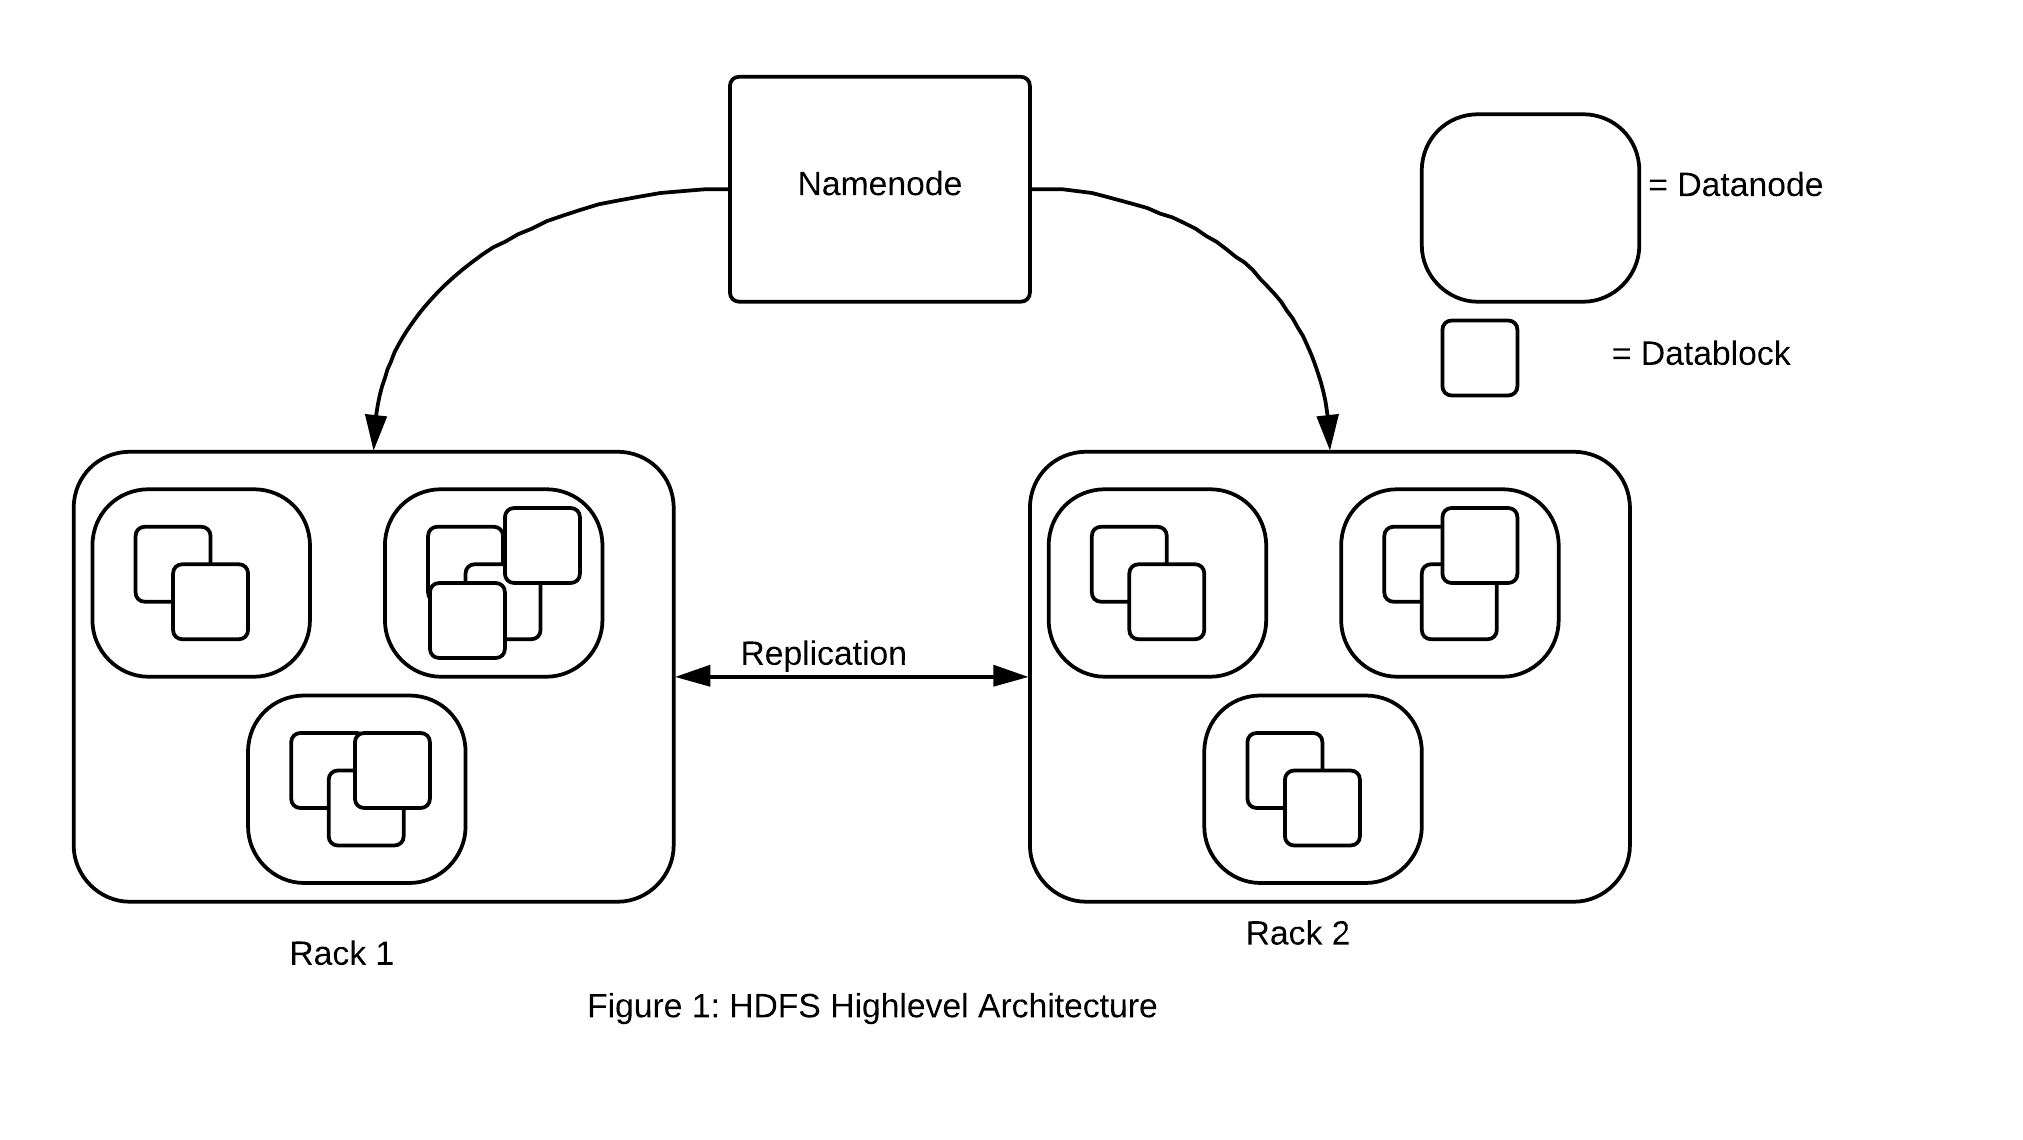
\includegraphics[width=\70]{images/HDFSArchitecture.png}
This diagram shows how a large file gets distributed across 
different datablocks in different racks and the replication of
datanodes between racks.
 
A default replication value of 3 means that data is stored on three
datanodes: two on the same rack, and one on a different rack. A
datanode resides on a rack and there can be multiple data nodes in a
rack. There’s a built-in coordination among the data nodes to
rebalance data, to move data copies around and maintain the
replication of data high. This builtin replication helps make the
data highly available. And because HDFS is not fully POSIX-compliant,
the file-system has increased performance for data throughput~\cite{hid-sp18-506-hdfs2}.

However, having only one namenode in the cluster can be a single
point of failure of the system. But starting version in 2.0, the
nameNode could be manually fail-over onto a backup. This version
also paved the way for developing automatic failovers in the
subsequent versions.

When a client requests for a file, the namecode knows which nodes the
data is stored and the request is then processed by the multiple
nodes in parallel. When a node is unavailable the other nodes can
take its place since the data is replicated across the different
nodes. 

\section {Conclusion}

Therefore, HDFS provides an efficient and reliable solution to
process large data files more efficiently while maintaining high
availability of data. By harnessing the  power of multiple machines
working in parallel to split the large data into blocks, process the
blocks simultaneously and replicate the blocks into different racks,
reading and writing are faster as well the recovering from failure
are much shorter.

\begin{acks}
  The authors would like to thank Dr.~Gregor~von~Laszewski for his
  support and suggestions to write this paper.
\end{acks}

\bibliographystyle{ACM-Reference-Format}
\bibliography{report} 
